% ==========
% CHAPTER 4
% ==========
\OpenGrid

\ParallelChapter
  {Reasoning with Number and Measurement}
  {Luận với số và đo lường}
  {}

\TriPara
  {
    \EN{Much of mathematics, particularly the domains of number and measurement, originated in efforts to quantify the world. Number and measurement, which receive substantial attention in kindergarten through grade 8, are foundational for high school mathematics; without reasoning skills in these areas, students will be limited in their reasoning in other areas of mathematics.}
  }
  {
    \VI{Phần lớn toán học, đặc biệt là hai mảng số và đo lường, bắt nguồn từ nỗ lực lượng hóa thế giới. Số và đo lường, vốn được chú trọng đáng kể từ mẫu giáo đến lớp 8, là nền tảng cho toán học trung học phổ thông; nếu không có kĩ năng luận trong hai mảng này, học sinh sẽ bị hạn chế trong việc luận ở những mảng khác của toán học.}
  }
  {
    \NOTE{Trong tiếng Anh, \emph{domain} và \emph{area} đều có thể dùng để chỉ một phạm vi nội dung của toán học, nhưng sắc thái của chúng không hoàn toàn trùng nhau. \emph{Domain} thường gợi một miền tương đối có ranh giới nhận diện được, còn \emph{area} là một cách gọi mềm và chung hơn cho một phạm vi hay một phần nội dung. Tuy vậy, sự khác biệt ấy không phải lúc nào cũng đủ rõ để chuyển thẳng sang tiếng Việt bằng hai nhãn cố định mà vẫn giữ được sự tự nhiên. Nếu cố tách riêng ở đây, bản dịch rất dễ trở nên nặng hoặc gượng, trong khi nguyên văn không đặt trọng tâm vào việc phân biệt thuật ngữ giữa \emph{domains} và \emph{areas}, mà vào việc nhấn mạnh số và đo lường là nền tảng, và từ hai mảng này năng lực luận mới có thể mở sang những mảng khác của toán học. Vì vậy, bản dịch chọn cách giản lược: ở vế đầu, dịch thẳng thành ``đặc biệt là số và đo lường''; về sau mới dùng ``hai mảng này'' và ``những mảng khác của toán học''. Cách xử lí ấy bỏ được sự gò ép thuật ngữ, giữ câu tiếng Việt mượt hơn, mà vẫn bảo toàn đúng ý chính của nguyên tác.}
  }

\TriPara
  {
    \EN{Key elements of reasoning and sense making with number and measurement include the following:
    \begin{itemize}
      \item \emph{Reasonableness of answers and measurements.} Judging whether a given answer or measurement has an appropriate order of magnitude, and whether it is expressed in appropriate units.
      
      \item \emph{Approximations and error.} Realizing that all real-world measurements are approximations and that unsuitably accurate values should not be used for real-world quantities; recognizing the role of error in subsequent computations with measurements.
      
      \item \emph{Number systems.} Understanding number-system properties deeply; extending number-system properties to algebraic situations.
      
      \item \emph{Counting.} Recognizing when enumeration would be a productive approach to solving a problem, and then using principles and techniques of counting to find a solution.
    \end{itemize}
    We address these key elements in more detail in the following sections.}
  }
  {
    \VI{Những yếu tố then chốt của luận và hiểu với số và đo lường gồm có:\vspace{\baselineskip}
    \begin{itemize}
      \item \emph{Tính hợp lí của đáp số và phép đo.} Đánh giá xem đáp số hoặc phép đo đã cho có bậc độ lớn thích hợp hay không, và có được biểu thị bằng đơn vị phù hợp hay không.\vspace{\baselineskip}

      \item \emph{Xấp xỉ và sai số.} Nhận ra rằng mọi phép đo trong thế giới thực đều là giá trị xấp xỉ, và không nên dùng những giá trị có độ chính xác không phù hợp cho các đại lượng thực tế; nhận ra vai trò của sai số trong những phép tính tiếp theo với các phép đo.

      \item \emph{Hệ thống số.} Hiểu sâu tính chất của hệ thống số; mở rộng tính chất của hệ thống số sang các tình huống đại số.
      
      \item \emph{Đếm.} Nhận ra khi nào liệt kê là cách tiếp cận hữu hiệu để giải bài toán, rồi vận dụng các nguyên lí và kĩ thuật đếm để tìm lời giải.
    \end{itemize}\vspace{\baselineskip}
    Chúng tôi sẽ trình bày chi tiết hơn các yếu tố then chốt này trong những phần tiếp theo.}
  }
  {
    \NOTE{Tác giả đang dựng khung cho toàn bộ phần bàn về số và đo lường bằng bốn yếu tố then chốt: đánh giá tính hợp lí, ý thức về xấp xỉ và sai số, hiểu cấu trúc của các hệ thống số, và nhận ra khi nào đếm là một con đường giải quyết thích hợp. Trọng tâm không nằm ở việc nêu thêm các mảng nội dung quen thuộc của chương trình, mà ở việc xác định những phương thức luận và hiểu cần hiện diện khi học số và đo lường. Nhờ đó, các phần sau của chương được đọc như sự triển khai của một khung năng lực, không phải như một danh sách chủ đề rời nhau.}
  }

\ParallelSection
  {Reasonableness of Answers and Measurements}
  {Tính hợp lí của đáp số và phép đo}
  {}

\TriPara
  {
    \EN{Students should possess ``number sense'' related to the base-ten numeration system. They should know that the leading, or leftmost, digit of a number accounts for most of the number, and that the digits to the right of the leading two or three digits of a measurement are ``loose change'' and are often insignificant. For example, although the U.S. Census Bureau Web site reports that the world population was 6,752,904,311 as of 9:48 a.m. on January 10, 2009, this number is only a rough estimate based on data provided from nations around the world. Indeed, one can often use round numbers to do approximate calculations that will yield simple but fairly accurate approximations of quantities of interest. See, for example, the comments of student 3 in example 1. This example also shows the importance of justifying one's answer and considering whether a solution makes sense and answers the question.}
  }
  {
    \VI{Học sinh cần có ``cảm thức số'' gắn với hệ ghi số thập phân. Các em cần biết rằng chữ số đứng đầu, hay chữ số ngoài cùng bên trái, chiếm phần lớn giá trị của một số, và rằng các chữ số nằm bên phải hai hoặc ba chữ số đầu của một phép đo chỉ là ``tiền lẻ'' và thường không đáng kể. Ví dụ, mặc dù trang web của Cục Thống kê Dân số Hoa Kì báo cáo rằng dân số thế giới tính đến 9:48 sáng ngày 10 tháng 1 năm 2009 là 6 752 904 311 người, con số này chỉ là ước tính thô dựa trên dữ liệu do các quốc gia trên thế giới cung cấp. Thật vậy, người ta thường có thể dùng số tròn để thực hiện phép tính xấp xỉ, từ đó thu được ước lượng đơn giản nhưng khá chính xác về đại lượng đang xét. Chẳng hạn, hãy xem nhận xét của Học sinh 3 trong Ví dụ 1. Ví dụ này cũng cho thấy tầm quan trọng của việc biện minh cho đáp án và xem xét liệu lời giải có hợp lí và có trả lời đúng câu hỏi hay không.}
  }{\NOTE{}}

\TriExample
  {Around the World}
  {
    \textbf{Task}

    Estimate the total surface area of the earth.

    \textbf{In the Classroom (Geometry Class)}

    \begin{scriptlist}
      \item [Teacher:] What would you predict the total surface area of the earth is?
      
      \item [Student 1:] Wow, I would have no idea. I'd guess either a million or maybe a billion square miles.
      
      \item [Student 2:] Well, it is a ball, which is basically a sphere. So if we knew the radius, I guess we could figure that out.
      
      \item [Teacher:] OK, to help you out, I'll tell you that its radius is about $4,000$ miles.
      
      \item [Student 2:] So then $A = 4\pi r^2$ , and we just need to plug the radius in.
      
      \item [Student 3:] If the radius is about $4$ thousand, then squaring will take us to about $16$ million. And $4\pi$ is a little more than $12$, and $12 \times 16 = 192$, so I'll guess maybe $200$ million square miles.
      
      \item [Student 4:] Yeah, that's decent, but why not just use the π-button on your calculator? That's what I did, and I got $201,061,930$.
      
      \item [Teacher:] So which do you think is the best estimate?
      
      \item [Student 4:] Mine, because it's most accurate.
      
      \item [Student 3:] But we don't know exactly what the radius of the earth is. Besides, the earth may not be exactly spherical. Your number is within $1$ percent of $200,000,000$, so I think $200,000,000$ is good enough.
    \end{scriptlist}\vspace{\baselineskip}

    \textbf{Key Elements of Mathematics}

    \begin{hanglist}
      \hangitem{Reasoning with Number and Measurement---Reasonableness of answers and measurements; Approximations and error}
    \end{hanglist}

    \textbf{Reasoning Habits}

    \begin{hanglist}
      \hangitem{Analyzing a problem---making preliminary deductions and conjectures}
      
      \hangitem{Reflecting on a solution---considering the reasonableness of a solution; justifying or validating a solution}
    \end{hanglist}
  }
  {Thế giới rộng nhường nào?}
  {
    \textbf{Nhiệm vụ}

    Ước tính tổng diện tích bề mặt Trái Đất.

    \textbf{Trong lớp học (Lớp Hình học)}

    \begin{scriptlist}
    \item [Giáo viên:] Các em dự đoán tổng diện tích bề mặt Trái Đất vào khoảng bao nhiêu?

    \item [Học sinh 1:] Ôi, em không có ý niệm gì cả. Em đoán hoặc một triệu, hoặc có khi một tỉ mile\footnote{Mile (mi): đơn vị đo độ dài trong hệ Mĩ; $1\;\text{mi}= 1.609344\;\text{k}m$.} vuông.

    \item [Học sinh 2:] À, Trái Đất giống một quả bóng, về cơ bản là hình cầu. Vậy nếu biết bán kính thì em nghĩ mình có thể tính ra.

    \item [Giáo viên:] Được, để hỗ trợ các em, tôi cho biết bán kính Trái Đất vào khoảng $4\,000$ mile.

    \item [Học sinh 2:] Vậy thì $A = 4\pi r^2$, chúng ta chỉ cần thay bán kính vào thôi.

    \item [Học sinh 3:] Nếu bán kính cỡ $4$ nghìn, thì bình phương lên sẽ vào khoảng $16$ triệu. Mà $4\pi$ lớn hơn $12$ một chút, còn $12 \times 16 = 192$, nên mình đoán chắc khoảng $200$ triệu mile vuông.

    \item [Học sinh 4:] Ừ, cách đó cũng ổn, nhưng sao không bấm luôn nút $\pi$ trên máy tính? Mình đã làm vậy và được $201\,061\,930$.

    \item [Giáo viên:] Vậy theo các em, đâu là ước lượng tốt nhất?

    \item [Học sinh 4:] Của em, vì nó chính xác nhất.

    \item [Học sinh 3:] Nhưng chúng ta không biết chính xác bán kính Trái Đất là bao nhiêu. Hơn nữa, Trái Đất cũng chưa chắc là một khối cầu hoàn hảo. Con số của bạn lệch chưa đến $1$ phần trăm so với $200\,000\,000$, nên mình nghĩ $200\,000\,000$ là đủ tốt rồi.
    \end{scriptlist}

    \textbf{Các yếu tố then chốt của toán học}

    \begin{hanglist}
      \hangitem{Luận với số và đo lường---Tính hợp lí của đáp số và phép đo; Xấp xỉ và sai số}
    \end{hanglist}\vspace{\baselineskip}

    \textbf{Thói quen luận}

    \begin{hanglist}
      \hangitem{Phân tích bài toán---đưa ra suy diễn và phỏng đoán sơ bộ}
      
      \hangitem{Phản tư về lời giải---xem xét tính hợp lí của lời giải; biện minh hoặc kiểm chứng lời giải}
    \end{hanglist}
  }
  {
    Ví dụ này làm lộ ra sự thật rất quan trọng khi học toán: con số có nhiều chữ số hơn chưa chắc là ước lượng tốt hơn. Học sinh 4 dùng công thức $A = 4\pi r^2$ và máy tính để cho ra kết quả $201\,061\,930$, nên em ấy tin rằng đáp số này là ``chính xác nhất''. Nhưng Học sinh 3 nhận ra rằng dữ kiện đầu vào chỉ là giá trị gần đúng: bán kính Trái Đất được cho là ``khoảng $4\,000$ mile'', chứ không phải trị số chính xác; hơn nữa, Trái Đất cũng không phải khối cầu hoàn hảo. Vì vậy, kết quả có quá nhiều chữ số dễ tạo ra \emph{ảo giác chính xác}, trong khi mức độ chắc chắn của dữ kiện ban đầu không cho phép khẳng định đến từng đơn vị như thế. Trong ngữ cảnh này, đáp số khoảng $200$ triệu mile vuông lại là ước lượng hợp lí hơn, vì nó phù hợp với độ chính xác thực sự của dữ kiện và mô hình đang dùng.

    Điểm đáng chú ý ở ví dụ này là lớp học không dừng lại ở việc ``tính ra đáp số'', mà đi tiếp đến câu hỏi: đâu là ước lượng tốt nhất, và vì sao? Chính câu hỏi đó buộc học sinh chuyển từ thao tác tính toán sang suy xét về tính hợp lí của kết quả. Từ dự đoán rất thô ban đầu của Học sinh 1, lớp học dần đi qua các bước: nhận diện mô hình hình học thích hợp, sử dụng công thức, ước lượng theo bậc độ lớn, rồi cuối cùng phản tư về sai số và giới hạn của mô hình. Bởi vậy, ví dụ này minh họa rất rõ hai yếu tố của luận với số và đo lường: tính hợp lí của đáp số và vai trò của xấp xỉ, sai số. Đồng thời, nó cũng cho thấy luận toán học không chỉ nằm ở chỗ tính đúng, mà còn ở chỗ biết đánh giá xem kết quả đáng tin đến mức nào trong bối cảnh đã cho.

    Nếu nói ngắn gọn hơn, hạt nhân sư phạm của ví dụ là câu này: \emph{trong bài toán gắn với đo lường thực tế, độ tinh vi của đáp số phải tương xứng với độ tin cậy của dữ kiện}. Ở đây, chính Học sinh 3 mới là người nhìn ra điều đó rõ nhất.
  }

\TriPara
  {
    \EN{Number sense lays an important foundation for learning high school mathematics. The National Mathematics Advisory Panel (2008) noted that ``poor number sense interferes with learning algorithms and number facts and prevents the use of strategies to verify if solutions to problems are reasonable'' (p. 27). The report goes on to identify the importance of developing both conceptual and procedural knowledge of fractions for progress in mathematics and the ``pervasive difficulties'' (p. 28) that students have. Although instructional time precludes reteaching the number concepts and operations that students should already have learned as they enter high school, attention to number sense can profitably be integrated into instructional objectives at the high school level. For example, teachers might routinely ask students to decide whether an answer to a given computation has the right order of magnitude, or what degree of accuracy would be appropriate in an answer, and to then state the reasoning for their judgment.}
  }
  {
    \VI{Cảm thức số đặt nền tảng quan trọng cho việc học toán ở bậc trung học phổ thông. National Mathematics Advisory Panel (2008) ghi nhận rằng ``cảm thức số yếu gây cản trở việc học thuật toán và các kết quả số học cơ bản, đồng thời ngăn học sinh sử dụng chiến lược để kiểm tra xem lời giải của một bài toán có hợp lí hay không'' (p. 27). Báo cáo tiếp tục chỉ ra tầm quan trọng của việc phát triển cả kiến thức khái niệm lẫn kiến thức thủ tục về phân số đối với tiến bộ trong toán học, cũng như ``những khó khăn phổ biến'' (p. 28) mà học sinh gặp phải. Mặc dù thời lượng dạy học không cho phép dạy lại các khái niệm và phép tính về số mà học sinh đáng lẽ đã học trước khi vào trung học phổ thông, việc chú trọng cảm thức số vẫn có thể được tích hợp hiệu quả vào mục tiêu dạy học ở bậc trung học phổ thông. Chẳng hạn, giáo viên có thể thường xuyên yêu cầu học sinh xác định xem kết quả của một phép tính đã cho có đúng bậc độ lớn hay không, hoặc mức độ chính xác nào là thích hợp đối với một đáp số, rồi trình bày phần luận làm căn cứ cho phán đoán ấy.}
  }{\NOTE{}}

\TriPara
  {
    \EN{In this publication, we call for the extension of ``number sense'' at the high school level to new sets of numbers and situations. Students should develop intuitions about situations involving radicals and negative and fractional exponents. For example, when calculating $12^\frac{3}{2}$, a student might reason that because $12$ is between $9$ and $16$, $12^\frac{1}{2}$ must be between $3$ and $4$.  Because $12^\frac{3}{2}=12^1\cdot 12^\frac{1}{2}$, the answer should be between $36$ and $48$. Thus, if a student enters ``{\normalfont\detokenize{12^3/2}}'' into his or her calculator to compute $12^\frac{3}{2}$ and gets an answer of $864$, he or she should immediately realize that a mistake has been made.}
  }
  {
    \VI{Trong tài liệu này, chúng tôi kêu gọi mở rộng ``cảm thức số'' ở bậc trung học phổ thông sang các tập số mới và tình huống mới. Học sinh cần phát triển trực giác về những tình huống liên quan đến căn thức, số mũ âm và số mũ phân số. Chẳng hạn, khi tính giá trị của $12^{\frac{3}{2}}$, học sinh có thể lập luận rằng vì $12$ nằm giữa $9$ và $16$, nên $12^{\frac{1}{2}}$ phải nằm giữa $3$ và $4$. Vì $12^{\frac{3}{2}} = 12^1 \cdot 12^{\frac{1}{2}}$, nên kết quả phải nằm giữa $36$ và $48$. Do đó, nếu học sinh nhập ``{\normalfont\detokenize{12^3/2}}'' vào máy tính để tính $12^{\frac{3}{2}}$ và nhận được kết quả $864$, em đó phải lập tức nhận ra rằng đã có sai sót.}
  }{\NOTE{}}

\TriPara
  {
    \EN{When working with measurements, students should have a sense of what units are appropriate for the solution to a problem. Example 2 presents a class discussion in which the teacher facilitates a comparison of different solutions to a problem. To help students interpret how their solutions might answer the problem, the teacher asks them to write out a formal response to the problem.}
  }
  {
    \VI{Khi làm việc với phép đo, học sinh cần có cảm nhận về đơn vị phù hợp cho đáp số của bài toán. Ví dụ 2 trình bày một cuộc thảo luận trên lớp, trong đó giáo viên dẫn dắt học sinh so sánh những lời giải khác nhau cho cùng một bài toán. Để giúp học sinh diễn giải cách lời giải của mình có thể trả lời bài toán, giáo viên yêu cầu các em viết ra một câu trả lời chính thức cho bài toán.}
  }{\NOTE{}}

\TriExample
  {Fuel for Thought}
  {
    \textbf{Task}

    A teacher gives her students the following quiz taken from an article in the New York Times (Chang 2008) and asks them to explain their reasoning:

    \textbf{Quiz time:} Which of the following would save more fuel?

    \begin{enumerate}
      \item [(a)] Replacing a compact car that gets $34$ miles per gallon (MPG) with a hybrid that gets $54$ MPG.
      
      \item [(b)] Replacing a sport utility vehicle (SUV) that gets $18$ MPG with a sedan that gets $28$ MPG.\vspace{\baselineskip}
      
      \item [(c)] Both changes save the same amount of fuel.
    \end{enumerate}

    \textbf{In the Classroom (First-Year Algebra)}

    The teacher collects the quizzes and asks two of her students to share their answers with the class. The first student responds:

    \begin{quote}
      I would say the correct answer is (a). My reasoning is that the change from $34$ MPG to $54$ is an increase of about $59$ percent, but the $18$ to $28$ MPG change is an increase of only about $56$ percent.
    \end{quote}

    The second student responds:

    \begin{quote}
      I thought about how much gas it would take to make a $100$-mile trip.

      \emph{Considering the compact car:}

      $100$ miles/$5$4 MPG = $1.85$ gallons used.

      $100$ miles/$34$ MPG = $2.94$ gallons used.

      So switching from a $3$4 MPG to a $54$ MPG car would save $1.09$ gallons of gas.

      \emph{Looking at the SUV:}

      $100$ miles/$28$ MPG = $3.57$ gallons used.

      $100$ miles/$18$ MPG = $5.56$ gallons used.

      So switching from an $18$ MPG car to a $28$ MPG car saves $1.99$ gallons of gas every $100$ miles. That means you are actually saving more gas by replacing the SUV.
    \end{quote}

    The teacher then asks the class to compare these two responses. After a spirited debate among students who had chosen each of the answers, the class reaches a consensus that both responses had merit, depending on how the problem is interpreted. Although the fuel efficiency increased slightly more for the compact car, the owner would actually save more gallons of gasoline by replacing the SUV if both cars were driven the same number of miles.

    The teacher asks the class to explore the relationship of MPG with actual gasoline consumption. After the students work in small groups for a few minutes, the teacher asks one group to show the table of values and graph it has made, as shown below. They explain, ``You save less fuel as you go up another $5$ MPG over and over. So as we saw in the quiz, MPG can be a little confusing.''

    \begin{center}
      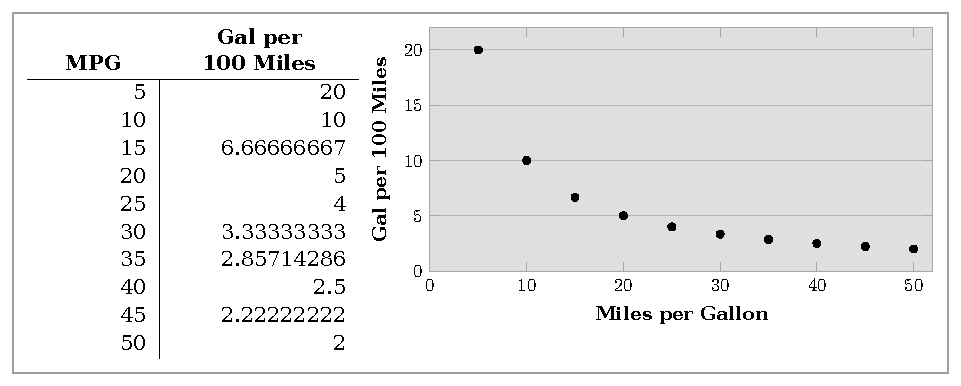
\includegraphics[width=.92\linewidth]{../figures/fhsm_2009_p24_f1.pdf}
    \end{center}

    The teacher then gives the class the article from the New York Times from which the quiz was taken to read for homework, along with some online comments from readers. She asks the students to analyze the arguments from the article in a brief essay and to propose what unit of measure they think will be useful for comparing the fuel consumption of cars.

    One group made this report: ``The low mileage cars offer more opportunities for savings because they are using so much gas. If you go from $10$ MPG to $20$ MPG, you go from using $10$ gallons for $100$ miles to $5$ gallons. You have saved $5$ gallons per hundred miles, and that is as much as you are using after the improvement. If you double the rate again to $40$ MPG, you will still use $2\tfrac{1}{2}$ gallons in $100$ miles, so you have only saved $2\tfrac{1}{2}$ gallons from the $20$ MPG amount or $7\tfrac{1}{2}$ gallons from the $10$ MPG amount. Even if you double again, to $80$ MPG, you will still use $1.25$ gallons, so you have only saved an additional $1.25$ gallons from the $40$ MPG amount. The point seems to be, the less you use, the less savings you have available. You can't save more than you use.''\vspace{3\baselineskip}

    \textbf{Key Elements of Mathematics}

    \begin{hanglist}
      \hangitem{Reasoning with Number and Measurement---Reasonableness of answers and measurements}

      \hangitem{Reasoning with Functions---Multiple representations of functions }
    \end{hanglist}

    \textbf{Reasoning Habits}

    \begin{hanglist}
      \hangitem{Analyzing a problem-seeking patterns and relationships}

      \hangitem{Reflecting on a solution---interpreting a solution; reconciling different approaches; refining arguments}
    \end{hanglist}
  }
  {Ngẫm về nhiên liệu}
  {
    \textbf{Nhiệm vụ}

    Một giáo viên đưa cho học sinh câu hỏi trắc nghiệm dưới đây, trích từ một bài báo trên New York Times (Chang 2008), và yêu cầu các em giải thích luận của mình:

    \textbf{Câu hỏi trắc nghiệm:} Trường hợp nào sau đây sẽ tiết kiệm được nhiều nhiên liệu hơn?

    \begin{enumerate}
      \item [(a)] Thay một xe cỡ nhỏ đi được $34$ mile trên mỗi gallon\footnote{Gallon (gal): đơn vị đo thể tích trong hệ Mĩ; $1\;\text{gal}=3.79\;\text{l}$.} (MPG) bằng một xe lai\footnote{Xe lai: cách dịch của \emph{hybrid car}, chỉ loại xe kết hợp động cơ đốt trong với động cơ điện để giảm mức tiêu thụ nhiên liệu.} đi được $54$ MPG.

      \item [(b)] Thay một xe thể thao đa dụng (SUV) đi được $18$ MPG bằng một xe du lịch bốn cửa\footnote{Xe du lịch bốn cửa: cách dịch mô tả của \emph{sedan}, chỉ kiểu xe thân kín, thường có bốn cửa, với khoang hành khách và khoang hành lí tách biệt.} đi được $28$ MPG.

      \item [(c)] Cả hai thay đổi đều tiết kiệm cùng một lượng nhiên liệu.
    \end{enumerate}

    \textbf{Trong lớp học (Đại số năm thứ nhất)}

    Giáo viên thu lại bài làm và mời hai học sinh chia sẻ đáp án của mình với cả lớp. Học sinh thứ nhất trả lời:

    \begin{quote}
      Em cho rằng đáp án đúng là (a). Phần luận của em là mức thay đổi từ $34$ MPG lên $54$ MPG tăng khoảng $59$ phần trăm, còn mức thay đổi từ $18$ MPG lên $28$ MPG chỉ tăng khoảng $56$ phần trăm.
    \end{quote}

    Học sinh thứ hai trả lời:

    \begin{quote}
      Em nghĩ đến việc cần bao nhiêu xăng để đi quãng đường $100$ mile.

      \emph{Xét chiếc xe cỡ nhỏ:}

      $100$ mile/$54$ MPG = $1.85$ gallon xăng đã dùng.

      $100$ mile/$34$ MPG = $2.94$ gallon xăng đã dùng. 

      Vậy chuyển từ xe $34$ MPG sang xe $54$ MPG sẽ tiết kiệm được $1.09$ gallon xăng.

      \emph{Xét chiếc SUV:}

      $100$ mile/$28$ MPG = $3.57$ gallon xăng đã dùng.

      $100$ mile/$18$ MPG = $5.56$ gallon xăng đã dùng.

      Vậy chuyển từ xe $18$ MPG sang xe $28$ MPG tiết kiệm được $1.99$ gallon xăng mỗi $100$ mile. Điều đó có nghĩa là thay chiếc SUV thực ra tiết kiệm được nhiều xăng hơn.
    \end{quote}

    Giáo viên yêu cầu cả lớp so sánh hai câu trả lời này. Sau cuộc tranh luận sôi nổi giữa những học sinh đã chọn mỗi đáp án, cả lớp đi đến thống nhất rằng cả hai câu trả lời đều có giá trị, tùy theo cách diễn giải bài toán. Mặc dù hiệu suất sử dụng nhiên liệu của xe cỡ nhỏ tăng nhiều hơn đôi chút, nhưng chủ xe thực ra sẽ tiết kiệm được nhiều gallon xăng hơn khi thay chiếc SUV, nếu cả hai xe đều đi cùng số mile như nhau.\vspace{\baselineskip}

    Giáo viên yêu cầu cả lớp khảo sát mối quan hệ giữa MPG và lượng xăng thực tế tiêu thụ. Sau khi học sinh làm việc theo nhóm nhỏ trong vài phút, giáo viên mời một nhóm trình bày bảng giá trị và đồ thị mà nhóm đã lập, như dưới đây. Các em giải thích: ``Khi cứ tăng thêm $5$ MPG hết lần này đến lần khác, lượng nhiên liệu tiết kiệm được lại ít đi. Vì vậy, như chúng ta đã thấy trong câu hỏi trắc nghiệm, MPG có thể hơi khó hiểu.''

    \begin{center}
      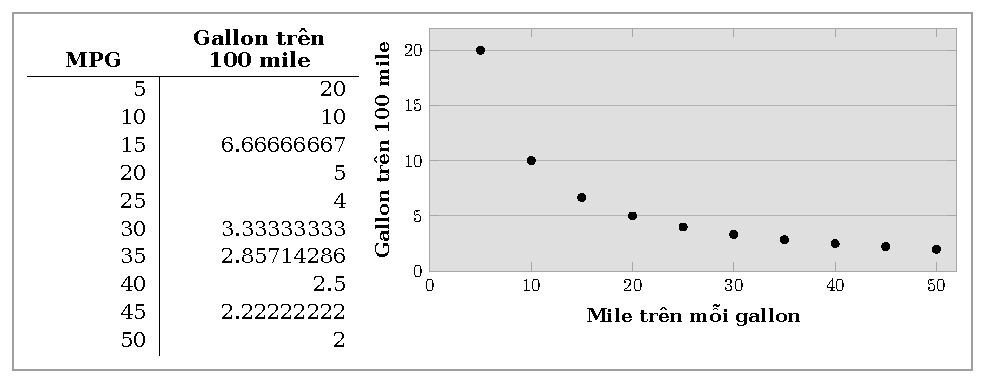
\includegraphics[width=.92\linewidth]{../figures/fhsm_2009_p24_f1_vi.pdf}
    \end{center}

    Sau đó, giáo viên giao cho cả lớp đọc ở nhà bài báo trên New York Times mà câu hỏi trắc nghiệm đã được lấy từ đó, cùng với một số bình luận trực tuyến của độc giả. Cô yêu cầu học sinh phân tích các lập luận trong bài báo bằng một bài viết ngắn và đề xuất đơn vị đo mà các em cho là hữu ích để so sánh mức tiêu thụ nhiên liệu của xe.

    Một nhóm đã viết báo cáo như sau: ``Những xe có mức tiết kiệm nhiên liệu thấp đem lại nhiều cơ hội tiết kiệm hơn, vì chúng đang dùng quá nhiều xăng. Nếu tăng từ $10$ MPG lên $20$ MPG, thì mức tiêu thụ giảm từ $10$ gallon cho mỗi $100$ mile xuống còn $5$ gallon. Như vậy, bạn tiết kiệm được $5$ gallon trên mỗi $100$ mile, và lượng tiết kiệm đó đúng bằng lượng xăng bạn còn dùng sau khi cải thiện. Nếu lại tăng gấp đôi mức này lên $40$ MPG, bạn vẫn sẽ dùng $2\tfrac{1}{2}$ gallon cho $100$ mile, nên bạn chỉ tiết kiệm thêm được $2\tfrac{1}{2}$ gallon so với mức $20$ MPG, hoặc tiết kiệm được $7\tfrac{1}{2}$ gallon so với mức $10$ MPG. Ngay cả khi lại tăng gấp đôi lần nữa, lên $80$ MPG, bạn vẫn còn dùng $1.25$ gallon, nên bạn chỉ tiết kiệm thêm được $1.25$ gallon so với mức $40$ MPG. Điểm chính dường như là: dùng càng ít thì phần còn có thể tiết kiệm thêm càng ít. Bạn không thể tiết kiệm nhiều hơn mức mình đang dùng.''

    \textbf{Các yếu tố then chốt của toán học}

    \begin{hanglist}
      \hangitem{Luận với số và đo lường---Tính hợp lí của đáp số và phép đo}\vspace{\baselineskip}
      
      \hangitem{Luận với hàm số---Nhiều biểu diễn của hàm số}
    \end{hanglist}

    \textbf{Thói quen luận}

    \begin{hanglist}
      \hangitem{Phân tích bài toán---tìm kiếm mẫu hình và quan hệ}

      \hangitem{Phản tư về lời giải---diễn giải lời giải; dung hòa những cách tiếp cận khác nhau; tinh chỉnh lập luận}
    \end{hanglist}
  }
  {
    \vspace{.5\baselineskip}
    Ví dụ này cho thấy cùng một tình huống thực tế có thể dẫn đến những câu trả lời khác nhau nếu người học chọn đại lượng so sánh khác nhau. Học sinh thứ nhất dựa vào mức tăng phần trăm của chỉ số MPG và kết luận rằng phương án (a) tốt hơn, vì $34$ lên $54$ MPG là mức tăng lớn hơn $18$ lên $28$ MPG. Cách tính này không sai, nhưng nó trả lời một câu hỏi khác: chỉ số MPG tăng theo tỉ lệ phần trăm bao nhiêu. Nếu hiểu câu hỏi theo nghĩa tự nhiên hơn---thay xe nào thực sự tiết kiệm được nhiều xăng hơn trên cùng một quãng đường---thì cần đổi từ MPG sang lượng xăng tiêu thụ. Khi cố định quãng đường ở $100$ mile, việc thay xe $18$ MPG bằng xe $28$ MPG giúp tiết kiệm khoảng $1.99$ gallon xăng, trong khi thay xe $34$ MPG bằng xe $54$ MPG chỉ tiết kiệm khoảng $1.09$ gallon.

    Điểm cốt lõi là: MPG cho biết một gallon xăng đi được bao nhiêu mile, còn câu hỏi tiết kiệm nhiên liệu lại đòi hỏi biết cần bao nhiêu gallon để đi cùng một số mile. Hai đại lượng này là nghịch đảo của nhau, nên chỉ nhìn vào mức tăng của MPG rất dễ gây ngộ nhận. Khi chuyển sang đại lượng gallon trên $100$ mile, ta thấy lượng xăng tiêu thụ giảm mạnh ở vùng MPG thấp rồi giảm chậm dần khi MPG tăng lên. Vì vậy, tăng thêm cùng một số MPG không đồng nghĩa với tiết kiệm thêm cùng một lượng nhiên liệu.

    Câu ``Bạn không thể tiết kiệm nhiều hơn mức mình đang dùng'' tuy hiển nhiên, nhưng giữ vai trò như điểm neo của lập luận. Nó buộc người học nhìn vào lượng xăng đang tiêu thụ trên cùng một quãng đường, thay vì chỉ nhìn vào mức tăng của chỉ số MPG. Một xe đang dùng nhiều xăng còn nhiều phần có thể giảm; một xe vốn đã tiết kiệm thì dù MPG tăng mạnh, lượng xăng có thể tiết kiệm thêm vẫn bị giới hạn bởi chính lượng xăng ít ỏi mà nó đang dùng. Theo nghĩa ấy, giá trị sư phạm của ví dụ không nằm ở bản thân phép tính, mà ở chỗ nó buộc học sinh xem lại đại lượng đang dùng để so sánh. Muốn đánh giá mức tiêu thụ nhiên liệu một cách có nghĩa, không thể chỉ nhìn trực tiếp vào chỉ số MPG, mà phải chọn đại lượng đo thật sự phù hợp với câu hỏi đang đặt ra.
  }

\ParallelSection
  {Approximations and Error}
  {Xấp xỉ và sai số}
  {}

\TriPara
  {
    \EN{Pure mathematics is exact, but when we want to apply it to the world, we must learn to cope with approximation. Numbers obtained through measurement rather than counting are subject to error, an important concept with which students need to struggle (Lehrer 2003). ``Error'' does not mean ``mistake''; it is the unavoidable inexactness that is inherent in all real-world situations. Many high school students have not grasped the significance of reporting their measure to the nearest unit or subunit of measurement, depending on the measuring device. Moreover, the accuracy of the measurement affects any results that are subsequently reported. When scientists give results based on measurements---often a mixture of direct and computed measures---they are careful to report the method(s) used to obtain them. Students should realize that in a measurement, the digits beyond the first few are likely not relevant and that they should be suspicious when they see measurements with many decimal places in news reports. Students should learn that the accuracy of a result can be more effectively specified using the idea of \emph{relative error}. Relative error is illustrated in example 3, as is the need for students to monitor their progress and adjust their strategies accordingly.}
  }
  {
    \VI{Toán học thuần túy là chính xác, nhưng khi muốn áp dụng nó vào thế giới, ta phải học cách xử lí xấp xỉ. Những con số thu được qua đo lường chứ không phải qua đếm đều chịu ảnh hưởng của sai số, một khái niệm quan trọng mà học sinh cần vật lộn để hiểu (Lehrer 2003). ``Sai số'' không có nghĩa là ``lỗi sai''; đó là độ không chính xác không thể tránh khỏi, vốn hiện diện trong mọi tình huống thực tế. Nhiều học sinh trung học phổ thông chưa nắm được ý nghĩa của việc báo cáo số đo đến đơn vị gần nhất hoặc đơn vị con gần nhất, tùy theo dụng cụ đo. Hơn nữa, độ chính xác của phép đo ảnh hưởng đến mọi kết quả được báo cáo về sau. Khi các nhà khoa học đưa ra kết quả dựa trên phép đo---thường là sự kết hợp giữa số đo trực tiếp và số đo tính toán---họ cẩn thận báo cáo phương pháp đã dùng để thu được các kết quả ấy. Học sinh cần nhận ra rằng trong một phép đo, các chữ số sau vài chữ số đầu thường không còn liên quan nhiều, và các em nên biết nghi ngờ khi thấy số đo có nhiều chữ số thập phân trong bản tin. Học sinh cần biết rằng độ chính xác của một kết quả có thể được mô tả hiệu quả hơn bằng ý tưởng \emph{sai số tương đối}. Sai số tương đối được minh họa trong Ví dụ 3, cùng với nhu cầu học sinh phải theo dõi tiến trình của mình và điều chỉnh chiến lược cho phù hợp.}
  }{\NOTE{}}

\TriExample
  {Around Pi}
  {
    \textbf{Task}

    Although we know that $\pi$ is an irrational number, we often use such approximations as $3.14$ or $22/7$. How much error are we introducing by using such an approximation? Find an upper bound for the relative error, and illustrate with a specific example.

    \textbf{In the Classroom (Second-Year Algebra)}

    Helping students move beyond the notion of error as a mistake is an important part of the sense-making process for a productive discussion of error. Students may view error as \emph{how far they are from a correct answer}. The teacher can build on this view to discus \emph{error} as the difference between an approximation $(v)$ and the ``real'' value $(V)$, and \emph{absolute error} as the absolute value or magnitude of the error, $\lvert V - v\rvert$. Developing an understanding of \emph{relative error} as a percent of the ``real'' value can help students make sense of the formula for relative error, $\frac{\lvert V-v\rvert}{V}$. To better understand his students' progress in understanding relative error, a teacher assigns the ``Around Pi'' task as an in-class assessment to be completed individually. One student's response follows, with the teacher's comments in the margin:\vspace{.5\baselineskip}

    \begin{quotation}
      I usually use $3.14$, so I decided to try that in the formula. But when I tried to figure out $\lvert V-v\rvert$, I got confused since we don't have an actual value for $V$ ($\pi$). But then I got this idea that I can be sure it is less than $.0016$, since $\pi<3.14159\dots$. So then I thought about $\frac{\lvert V-v\rvert}{V}$. We still don't know what $\pi$ is, but since $V$ is in the denominator, I'll pick something less than $V$, which would be $3.1415$. So $\frac{.0016}{3.1415}=9.0931\times 10^{-4}$. That's really small! Then I tried this with the area of a circle, with radius $5$, using $3.14$ and the $\pi$-button on my calculator, and it was only off by about $.0399$, so I guess that's pretty good!
      
      \begin{scriptlist}
        \item[Teacher:] Great idea! But you could explain this a little more fully.\vspace{\baselineskip}
        
        \item[Teacher:] Why did you change to less? Why was that important? Is this the exact value? Continue your argument using bounds. Is this relative error? Have you really mabd your point with this example? How does using the $\pi$-button relate to the value of $V$?
      \end{scriptlist}
      \end{quotation}\vspace{5.5\baselineskip}

    \textbf{Key Elements of Mathematics}

    \begin{hanglist}
      \hangitem{Reasoning with Number and Measurement---Approximations and error}
    \end{hanglist}

    \textbf{Reasoning Habits}

    \begin{hanglist}
      \hangitem{Analyzing a problem---defining relevant variables and conditions}

      \hangitem{Implementing a strategy---monitoring progress toward a solution}

      \hangitem{Reflecting on a solution---justifying or validating a solution; refining arguments}
    \end{hanglist}
  }
  {Số Pi dài - ngắn thế nào?}
  {
    \textbf{Nhiệm vụ}

    Mặc dù biết rằng $\pi$ là số vô tỉ, ta vẫn thường dùng các giá trị xấp xỉ như $3.14$ hoặc $22/7$. Khi dùng một giá trị xấp xỉ như vậy, ta đưa vào bao nhiêu sai số? Hãy tìm một cận trên cho sai số tương đối, và minh họa bằng một ví dụ cụ thể.

    \textbf{Trong lớp học (Đại số năm thứ hai)}

    Giúp học sinh vượt qua quan niệm xem sai số là lỗi sai là phần quan trọng của quá trình hiểu để có một thảo luận hiệu quả về sai số. Học sinh có thể xem sai số như \emph{khoảng cách giữa kết quả của mình và đáp án đúng}. Giáo viên có thể dựa trên cách nhìn này để thảo luận về \emph{sai số} như hiệu giữa giá trị xấp xỉ $(v)$ và ``giá trị thật'' $(V)$, và \emph{sai số tuyệt đối} như giá trị tuyệt đối hoặc độ lớn của sai số, $\lvert V - v\rvert$. Việc phát triển hiểu biết về \emph{sai số tương đối} như tỉ lệ phần trăm so với ``giá trị thật'' có thể giúp học sinh hiểu công thức sai số tương đối, $\frac{\lvert V - v\rvert}{V}$. Để hiểu rõ hơn tiến triển của học sinh trong việc hiểu sai số tương đối, giáo viên giao nhiệm vụ ``Số Pi dài - ngắn thế nào?'' như một bài đánh giá trên lớp, yêu cầu học sinh làm cá nhân. Sau đây là lời giải của một học sinh, kèm theo nhận xét bên lề của giáo viên:

    \begin{quote}
      Em thường dùng $3.14$, nên em quyết định thử dùng giá trị này trong công thức. Nhưng khi cố tính $\lvert V - v\rvert$, em bị rối vì ta không có giá trị thật sự $V$ (tức là $\pi$). Sau đó em nảy ra ý tưởng rằng ta có thể chắc chắn nó nhỏ hơn $.0016$, vì $\pi < 3.14159\dots$. Vậy nên em xét $\frac{\lvert V - v\rvert}{V}$. Ta vẫn chưa biết chính xác $\pi$ là bao nhiêu, nhưng vì $V$ nằm ở mẫu số, em sẽ chọn một số nhỏ hơn $V$, tức là $3.1415$. Như vậy $\frac{0.0016}{3.1415}=9.0931\times 10^{-4}$. Con số này rất nhỏ! Rồi em thử điều này với diện tích hình tròn bán kính $5$, dùng $3.14$ và dùng nút $\pi$ trên máy tính, thì kết quả chỉ lệch khoảng $0.0399$, nên em nghĩ như vậy là khá tốt!\vspace{\baselineskip}

      \begin{scriptlist}
        \item[Giáo viên:] Ý tưởng rất hay! Nhưng em có thể giải thích đầy đủ hơn một chút.
        
        \item[Giáo viên:] Tại sao em lại chuyển sang giá trị nhỏ hơn? Vì sao điều đó quan trọng? Đây có phải là giá trị chính xác không? Hãy tiếp tục lập luận bằng cách dùng các cận. Đây có phải là sai số tương đối không? Em đã thật sự làm rõ luận điểm của mình bằng ví dụ này chưa? Việc dùng nút $\pi$ trên máy tính liên quan thế nào đến giá trị $V$?
      \end{scriptlist}
    \end{quote}

    \textbf{Các yếu tố then chốt của toán học}

    \begin{hanglist}
      \hangitem{Luận với số và đo lường---Xấp xỉ và sai số}\vspace{\baselineskip}
    \end{hanglist}

    \textbf{Thói quen luận}

    \begin{hanglist}
      \hangitem{Phân tích bài toán---xác định cẩn thận biến và điều kiện thích đáng}

      \hangitem{Triển khai chiến lược---theo dõi tiến trình đi đến lời giải}

      \hangitem{Phản tư về lời giải---biện minh hoặc kiểm chứng lời giải; tinh chỉnh lập luận}
    \end{hanglist}
  }
  {
    \vspace{.5\baselineskip}
    Ví dụ 3 cho thấy sai số không được đặt ra như một mẩu kiến thức phụ kèm theo đo lường, mà như đối tượng của luận. Điều cần học không chỉ là hai khái niệm sai số tuyệt đối và sai số tương đối, mà là cách dùng bất đẳng thức và các cận để kiểm soát độ lớn của sai số ngay cả khi giá trị đang xét không được biết chính xác dưới dạng thập phân hữu hạn. Điểm đáng chú ý ở đây là học sinh đã đi đúng hướng khi tìm cách chặn sai số, nhưng lại bộc lộ lẫn lộn quan trọng trong cách chọn cận và trong cách diễn giải giá trị gần đúng của $\pi$. Sai sót ấy không làm hỏng giá trị của ví dụ; ngược lại, nó cho thấy hiểu trong toán không thể tách rời sự chính xác của ngôn ngữ và kí hiệu.

    Các nhận xét của giáo viên cũng bộc lộ rõ lập trường sư phạm của sách. Giáo viên không sửa hộ lời giải, mà buộc học sinh nói rõ vì sao chọn giá trị nhỏ hơn, vì sao cách chọn ấy quan trọng, và ví dụ tính diện tích hình tròn ở cuối thực sự chứng minh được điều gì. Trọng tâm vì thế không nằm ở việc chữa một lỗi riêng lẻ, mà ở việc đẩy học sinh đi tiếp từ trực giác ban đầu sang lập luận chặt hơn.

    Ví dụ này cũng làm sáng tỏ mối liên hệ giữa luận và hiểu. Khi so sánh kết quả dùng $\pi \approx 3.14$ với kết quả dùng nút $\pi$ trên máy tính, học sinh bắt đầu thấy sai số trong hằng số kéo theo sai khác ra sao trong đại lượng được tính. Nhờ đó, giá trị gần đúng không còn là con số thay thế tùy tiện, mà được hiểu trong quan hệ với mục đích tính toán và mức chính xác cần có.

    \begin{hanglist}
      \hangitem{\textbf{Bài tập.} Hãy sử dụng bất đẳng thức $3.1415<\pi<3.1416$ để xây dựng thêm một lập luận.}
    \end{hanglist}
  }

\ParallelSection
  {Number Systems}
  {Hệ thống số}
  {}

\TriPara
  {
    \EN{A solid understanding of number systems and their properties sets a foundation for meaningful development of algebra (Carraher and Schliemann 2007). Example 4 illustrates how an understanding of the distributive property with multidigit multiplication forms the basis for multiplication of polynomials; this point is further elaborated in example 6, ``Distribute Thoroughly''.}
  }
  {
    \VI{Hiểu vững hệ thống số và các tính chất của chúng đặt nền tảng cho sự phát triển có ý nghĩa của đại số (Carraher and Schliemann 2007). Ví dụ 4 minh họa cách hiểu tính chất phân phối của phép nhân các số nhiều chữ số tạo cơ sở cho phép nhân đa thức; điểm này sẽ được triển khai thêm trong Ví dụ 6, ``Phân phối triệt để''.}
  }{\NOTE{}}

\TriExample
  {A Model Idea}
  {
    \textbf{Background}

    The distributive property can be illustrated with an \emph{area model}. Take, for example, the product of $62$ and $43$. If each factor is written in expanded form, we have
    $$
      \begin{aligned}
        (62)(43)
          &=(60+2)(40+3)\\
          &=24(100)+18(10)+8(10)+6.
      \end{aligned}
    $$

    The figure below shows groups of $100$, $10$, and $1$ represented geometrically, helping students make sense not only of the distributive property but also of perfect squares and orders of magnitude.

    \begin{center}
      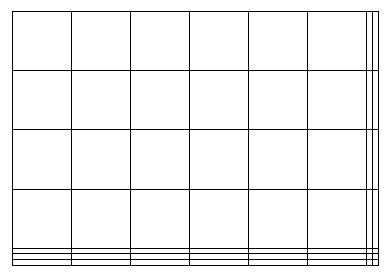
\includegraphics[width=.92\linewidth]{../figures/fhsm_2009_p27_1.pdf}
    \end{center}

    Once the concept of using area to model multiplication of integers has been established, ideally in kindergarten-grade 8, area models can help students make sense of many processes, such as multiplication of fractions and polynomials.

    \textbf{Task}

    The distributive property for multiplication of variables can be modeled for such expressions as $A(B + C)$. As shown in the figure that follows, $AB + AC = A(B + C)$.

    \begin{center}
      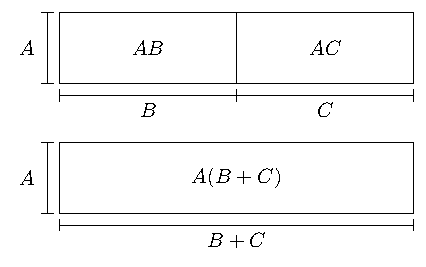
\includegraphics[width=.92\linewidth]{../figures/fhsm_2009_p28_1.pdf}
    \end{center}

    Create an area model for the product $(x + 3)(x + y + 5)$.

    \textbf{In the Classroom (First-Year Algebra)}

    Students could create area models by drawing on graph paper or using algebra tiles. Two possible area models are shown below. The first shows regions of area $x^2$, $xy$, $x$, $y$, and $1$. By counting the number of each type of region present (i.e., one group of $x^2$ , three groups of $y$, and so forth), students can make sense of what each term in the expansion of the product represents. The second model shows the area of each smaller rectangular region as the product of its dimensions. This type of area model illustrates that the sum of the smaller areas (products of terms) is equal to the area of the original factors, thus forming a connection with the area addition postulate. 

    \begin{center}
      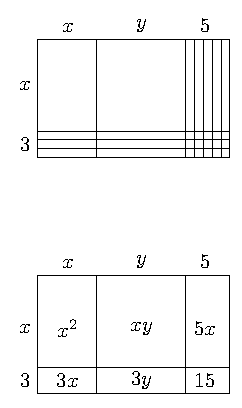
\includegraphics[width=.55\linewidth]{../figures/fhsm_2009_p28_2.pdf}
    \end{center}

    \textbf{Key Elements of Mathematics}

    \begin{hanglist}
      \hangitem{Reasoning with Number and Measurement---Number systems}
    \end{hanglist}

    \textbf{Reasoning Habits}

    \begin{hanglist}
      \hangitem{Analyzing a problem---identifying relevant concepts, procedures, or representations; applying previously learned concepts}

      \hangitem{Seeking and using connections}
    \end{hanglist}
  }
  {Những mảnh ghép đại số}
  {
    \textbf{Bối cảnh}

    Tính chất phân phối có thể được minh họa bằng một \emph{mô hình diện tích}. Chẳng hạn, xét tích của $62$ và $43$. Nếu mỗi thừa số được viết ở dạng khai triển, ta có
    $$
      \begin{aligned}
        (62)(43)
          &=(60+2)(40+3)\\
          &=24(100)+18(10)+8(10)+6.
      \end{aligned}
    $$

    Hình dưới đây biểu diễn hình học các nhóm $100$, $10$ và $1$, qua đó giúp học sinh hiểu không chỉ tính chất phân phối mà còn cả số chính phương và bậc độ lớn.\vspace{\baselineskip}

    \begin{center}
      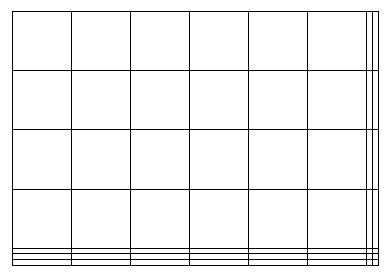
\includegraphics[width=.92\linewidth]{../figures/fhsm_2009_p27_1.pdf}
    \end{center}

    Một khi ý tưởng dùng diện tích để mô hình hóa phép nhân số nguyên đã được thiết lập, lí tưởng là từ mẫu giáo đến lớp 8, mô hình diện tích có thể giúp học sinh hiểu nhiều quá trình, chẳng hạn phép nhân phân số và phép nhân đa thức.

    \textbf{Nhiệm vụ}

    Tính chất phân phối của phép nhân với các biến có thể được mô hình hóa bằng những biểu thức như $A(B + C)$. Như hình vẽ tiếp theo cho thấy, $AB + AC = A(B + C)$.

    \begin{center}
      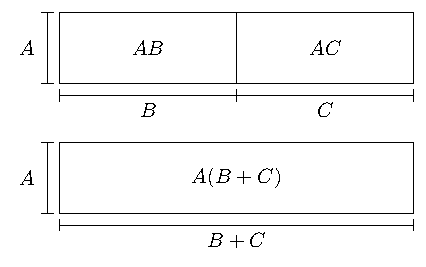
\includegraphics[width=.92\linewidth]{../figures/fhsm_2009_p28_1.pdf}
    \end{center}

    Hãy tạo một mô hình diện tích cho tích $(x + 3)(x + y + 5)$.

    \textbf{Trong lớp học (Đại số năm thứ nhất)}

    Học sinh có thể tạo mô hình diện tích bằng cách vẽ trên giấy kẻ ô hoặc dùng mảnh ghép đại số. Hai mô hình diện tích khả dĩ được minh họa dưới đây. Mô hình thứ nhất cho thấy các vùng có diện tích $x^2$, $xy$, $x$, $y$ và $1$. Bằng cách đếm số vùng thuộc mỗi loại, tức là một nhóm $x^2$, ba nhóm $y$, v.v., học sinh có thể hiểu mỗi hạng tử trong khai triển của tích biểu thị điều gì. Mô hình thứ hai thể hiện diện tích của từng vùng chữ nhật nhỏ dưới dạng tích hai kích thước của nó. Kiểu mô hình diện tích này minh họa rằng tổng diện tích các vùng nhỏ hơn, tức là các tích của các hạng tử, bằng diện tích ứng với các thừa số ban đầu, qua đó tạo kết nối với tiên đề cộng diện tích.

    \begin{center}
      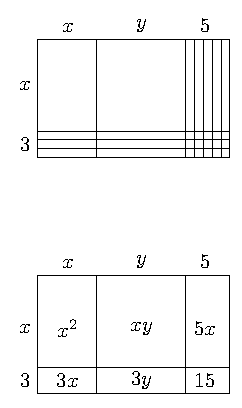
\includegraphics[width=.55\linewidth]{../figures/fhsm_2009_p28_2.pdf}
    \end{center}

    \textbf{Các yếu tố then chốt của toán học}

    \begin{hanglist}
      \hangitem{Luận với số và đo lường---Hệ thống số}
    \end{hanglist}\vspace{\baselineskip}

    \textbf{Thói quen luận}

    \begin{hanglist}
      \hangitem{Phân tích bài toán---xác định khái niệm, thủ tục, hoặc biểu diễn toán học thích đáng; vận dụng khái niệm đã học}

      \hangitem{Tìm kiếm và sử dụng kết nối}
    \end{hanglist}
  }{}

\ParallelSection
  {Counting}
  {Đếm}
  {}

\TriPara
{
  \EN{Counting principles and techniques, an important topic from discrete mathematics, have applications both within and outside mathematics. See example 20, ``What Are the Chances? Part A'' for an application of counting principles to probability models. Students need to understand the difference between counting the number of possible outcomes and enumerating all possible cases. For example, when rolling a pair of dice and summing the numbers of the topmost faces, eleven sums from $2$ to $12$ are possible. Yet not all sums are equally likely, because five ways exist to get $6$ ($1 + 5$, $2 + 4$, $3 + 3$, $4 + 2$, and $5 + 1$) but only one way to get $2$ $(1 + 1)$. Another important counting skill is understanding the difference between situations in which the order of events matters (e.g., the digits in a number) and situations in which order is irrelevant (e.g., membership on a committee, as in example 20, ``What Are the Chances? Part A'').}
}
{
  \VI{Các nguyên lí và kĩ thuật đếm, một chủ đề quan trọng của toán rời rạc, có ứng dụng cả trong lẫn ngoài toán học. Xem Ví dụ 20, ``Bao nhiêu khả năng? (A)'', để thấy một ứng dụng của các nguyên lí đếm vào mô hình xác suất. Học sinh cần hiểu khác biệt giữa việc đếm số kết quả có thể xảy ra và việc liệt kê tất cả trường hợp có thể xảy ra. Chẳng hạn, khi gieo hai xúc xắc rồi cộng số chấm trên hai mặt trên, ta có thể thu được mười một tổng từ $2$ đến $12$. Tuy nhiên, không phải tổng nào cũng có xác suất như nhau, vì có năm cách để được $6$ ($1 + 5$, $2 + 4$, $3 + 3$, $4 + 2$, và $5 + 1$), nhưng chỉ có một cách để được $2$ $(1 + 1)$. Một kĩ năng đếm quan trọng khác là hiểu khác biệt giữa tình huống mà thứ tự sự kiện có ý nghĩa (chẳng hạn, các chữ số trong một số) và tình huống mà thứ tự không quan trọng (chẳng hạn, thành phần của một ủy ban, như trong Ví dụ 20, ``Bao nhiêu khả năng? (A)'').}
}{\NOTE{}}

\TriPara
{
  \EN{A solid understanding of number and measurement continues to be important at the high school level because it provides the foundation for reasoning about other mathematical concepts. Helping students make sense of these essential ideas will ease their transition to more abstract topics.}
}
{
  \VI{Hiểu vững số và đo lường vẫn giữ vai trò quan trọng ở bậc trung học phổ thông, vì nó cung cấp nền tảng cho việc luận về các khái niệm toán học khác. Giúp học sinh hiểu những ý tưởng thiết yếu này sẽ làm cho quá trình chuyển sang các chủ đề trừu tượng hơn trở nên nhẹ nhàng hơn.}
}{\NOTE{}}

\CloseGrid